% Python4Physics 2025 Final Report
% Author: Arnav Kapoor
% Email: arnavkapoor23@iiserb.ac.in
% License: CC BY 4.0 (https://creativecommons.org/licenses/by/4.0/)
% 
% This LaTeX file is intended for public sharing on GitHub as part of the Python4Physics 2025 program submission.
% To compile: pdflatex Report_short.tex
% All figures are in the ../figures/ directory.
% Contributions, forks, and feedback are welcome!

\documentclass[12pt]{article}
\usepackage{graphicx}
\usepackage{amsmath}
\usepackage{hyperref}
\usepackage{geometry}
\geometry{margin=1in}
\title{Python4Physics 2025 -- Final Report}
\author{Arnav Kapoor}
\date{}
\begin{document}
\maketitle
\noindent Email: \texttt{arnavkapoor23@iiserb.ac.in}

\section*{Introduction}
The Python4Physics 2025 program was an enriching experience that deepened my understanding of both physics and scientific computing. This report summarizes the key concepts I learned, projects I enjoyed, and insights gained from lectures and guest presentations.

\section*{Program Highlights}
\begin{itemize}
  \item \textbf{Python Basics and Plotting:} Learned Python syntax, Jupyter notebooks, and matplotlib for visualizing mathematical functions.
  \item \textbf{Arrays, Data Structures, and File I/O:} Practiced with numpy arrays, lists, dictionaries, and saving/loading data for reproducibility.
  \item \textbf{Probability, Statistics, and Monte Carlo:} Generated random numbers, visualized distributions, and estimated $\pi$ using Monte Carlo methods.
  \item \textbf{Physics Simulations:} Modeled projectile motion and orbits, connecting physical principles with computational models.
  \item \textbf{Project Work and Collaboration:} Worked on a capstone project, collaborated with peers, and presented findings.
\end{itemize}


\section*{Key Figures}
\begin{center}
\setlength{\tabcolsep}{8pt}
\renewcommand{\arraystretch}{1.2}
\begin{tabular}{cc}
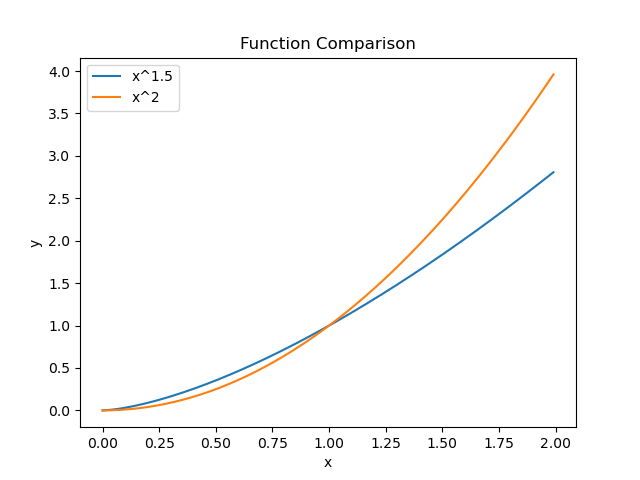
\includegraphics[width=0.35\textwidth]{../figures/Figure_1.png} &
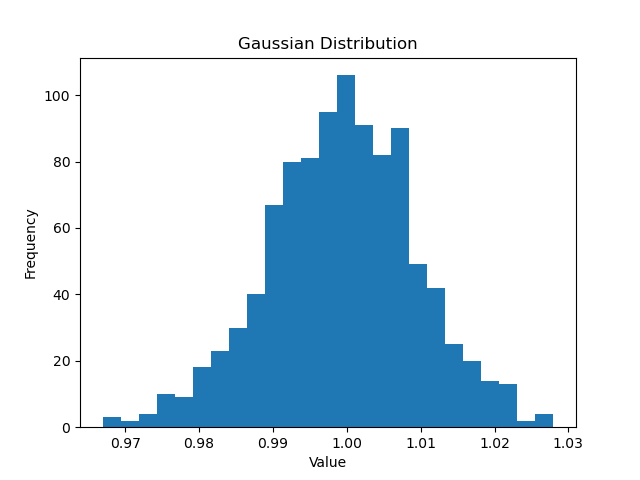
\includegraphics[width=0.35\textwidth]{../figures/Figure_2.png} \\
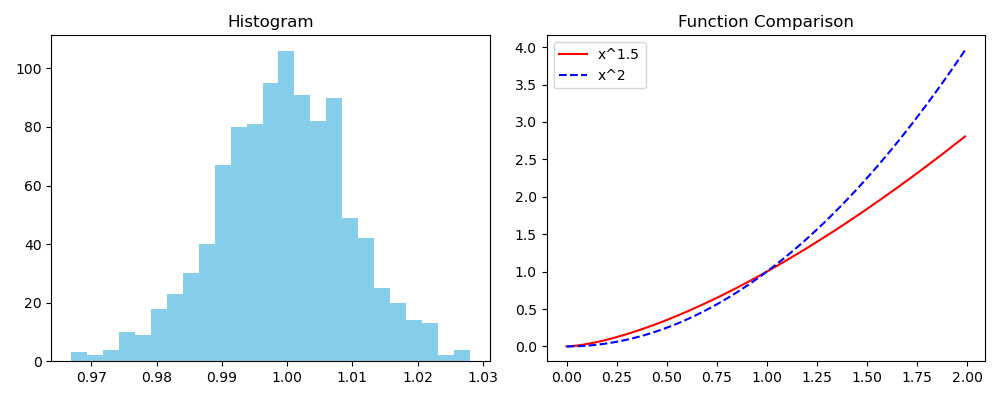
\includegraphics[width=0.35\textwidth]{../figures/Figure_3.png} &
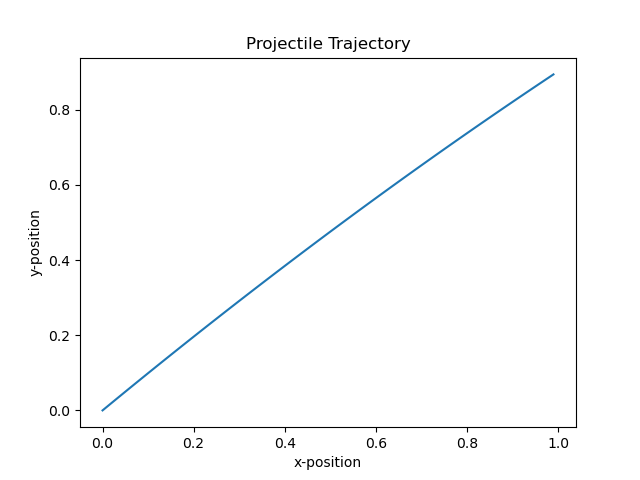
\includegraphics[width=0.35\textwidth]{../figures/Figure_4.png} \\
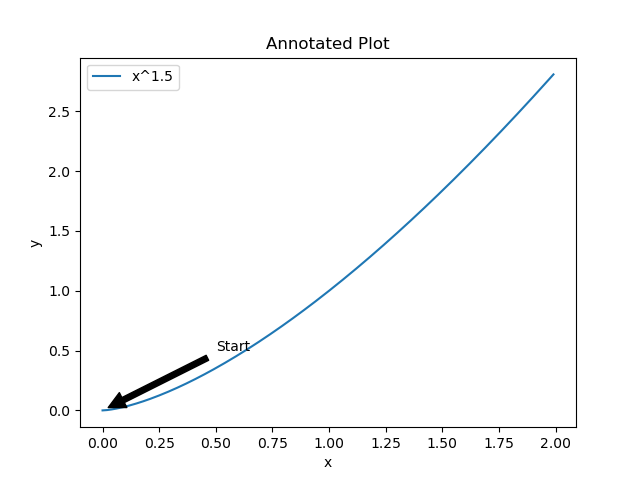
\includegraphics[width=0.35\textwidth]{../figures/Figure_5.png} &
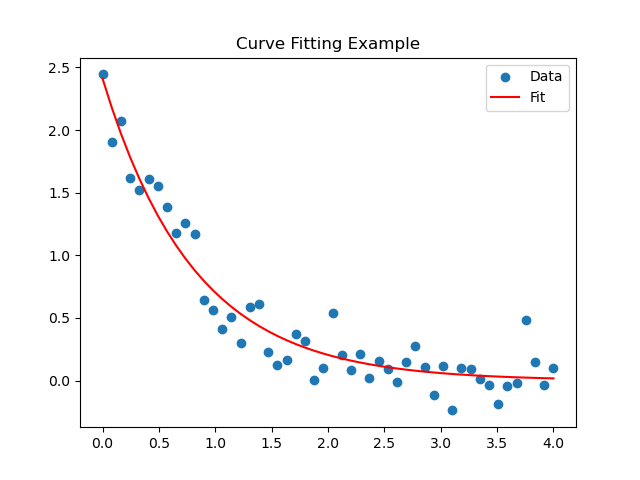
\includegraphics[width=0.35\textwidth]{../figures/Figure_6.png} \\
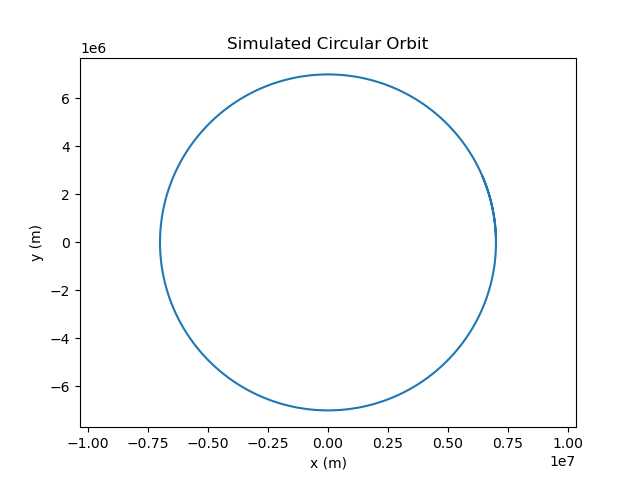
\includegraphics[width=0.35\textwidth]{../figures/Figure_7.png} &
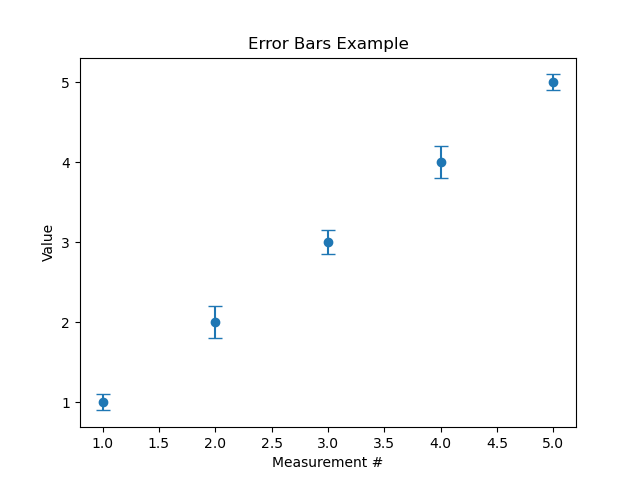
\includegraphics[width=0.35\textwidth]{../figures/Figure_8.png} \\
\end{tabular}
\end{center}

\noindent\textbf{Sample Code:}
\begin{verbatim}
import numpy as np
import matplotlib.pyplot as plt
x = np.arange(0, 2, 0.01)
def f1(x): return np.power(x, 1.5)
def f2(x): return np.power(x, 2)
plt.plot(x, f1(x), label='x^1.5')
plt.plot(x, f2(x), label='x^2')
plt.legend()
plt.show()
\end{verbatim}


\section*{Daily Highlights}
\begin{itemize}
  \item \textbf{Day 1: Introduction to Python and Plotting} -- Learned the basics of Python syntax and Jupyter notebooks. Explored data visualization with matplotlib, creating plots of mathematical functions and customizing their appearance.
  \item \textbf{Day 2: Arrays, Lists, and Data Structures} -- Gained experience with numpy arrays and Python lists, understanding their differences and use cases. Practiced manipulating arrays and performing vectorized operations for efficient computation.
  \item \textbf{Day 3: Probability and Random Numbers} -- Studied the generation of random numbers and their applications in simulations. Implemented Monte Carlo methods to estimate mathematical constants such as $\pi$.
  \item \textbf{Day 4: Statistics and Distributions} -- Learned about Gaussian (normal) distributions and how to generate and visualize them in Python. Used histograms to analyze the distribution of simulated data and compared it to theoretical curves.
  \item \textbf{Day 5: Data Handling and File I/O} -- Practiced saving and loading data using numpy's file I/O functions. Understood the importance of reproducibility and data management in scientific research.
  \item \textbf{Day 6: Advanced Plotting and Data Analysis} -- Created multi-panel plots and explored advanced features of matplotlib. Analyzed real and simulated datasets, extracting meaningful statistics and trends.
  \item \textbf{Day 7: Physics Simulations -- Projectile Motion} -- Modeled projectile motion using Python, varying initial conditions and visualizing trajectories. Connected physical principles with computational models to deepen understanding of kinematics.
  \item \textbf{Day 8: Project Work and Collaboration} -- Worked on a capstone project, applying skills learned throughout the program to a larger problem. Collaborated with peers, shared code, and presented findings to the group.
  \item \textbf{Day 9: Guest Lectures and Research Applications} -- Attended guest lectures on topics such as computational astrophysics and data science in physics. Learned how Python is used in cutting-edge research and discussed career pathways in computational science.
\end{itemize}

\section*{Reflections and Insights}
The program’s structure, combining lectures, coding exercises, and guest presentations, provided a holistic learning environment. I enjoyed the hands-on projects and the opportunity to collaborate with peers. The guest lectures, especially on computational astrophysics, inspired me to apply computational tools in future research.

\section*{Future Applications}
I plan to use the skills gained in Python4Physics in my future coursework and research. Whether analyzing experimental data, simulating physical systems, or visualizing results, I now feel confident in my ability to use Python as a powerful tool for scientific inquiry. I am also motivated to continue learning about advanced topics such as machine learning and computational modeling.

\section*{Conclusion}
Python4Physics 2025 has equipped me with practical skills in scientific programming and a deeper appreciation for computational physics. I am grateful for the opportunity to participate and look forward to applying these skills in future academic and research endeavors.

\vspace{1em}
\noindent\textbf{Thank you to the instructors, guest speakers, and fellow participants for making this a memorable and impactful experience.}

\end{document}
